\chapter{Introducción}
Primeramente hay que entender que es el Lenguaje de Programación \textit{Ensamblador}. Para ello hay que entender los niveles de los lenguajes del computador.
\section{Entendiendo los Niveles de Lenguajes de Programación}
Solo hay un lenguaje de programación que cualquier computadora puede entender y ejecutar: su propio código de máquina, \textit{binario nativo}. Este es el nivel de lenguaje más bajo posible en el cual se puede escribir un programa de computadora. Se dice que todos los otros idiomas son de nivel alto o bajo de acuerdo con cuán cerca se puede decir que se asemejan al código de la máquina.

\begin{figure}[h]
\centering
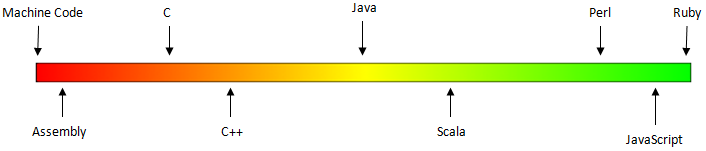
\includegraphics[scale=0.5]{Niveles}
\captionsetup{justification=centering}
\caption[caption]{\footnotesize Niveles de Programación en el Computador. \\ \textbf{Fuente:} \texttt{http://www.codecommit.com/blog/java/defining-high-mid-and-low-level-languages}}
\end{figure}
Con esta gráfica podemos tener una idea de que tan bajo se encuentra el lenguaje de programación Ensamblador en las computadoras. Es por esto que, a diferencia de un lenguaje de alto nivel que es portable a travez de multiples arquitecturas y requieren de un \textit{interpreter} o un \textit{compilador}, el lenguaje ensamblador es especifico a un tipo de arquitectura y sistema operativo. (En el curso usamos la arquitectura 80x86, IA32).
\subsection{Representación de Datos en el computador}
Teniendo algunos conceptos iniciales, algo que es importante de conocer, es la forma en como la computadora manejan datos de distinto tipo.
\begin{figure}[h]
\centering
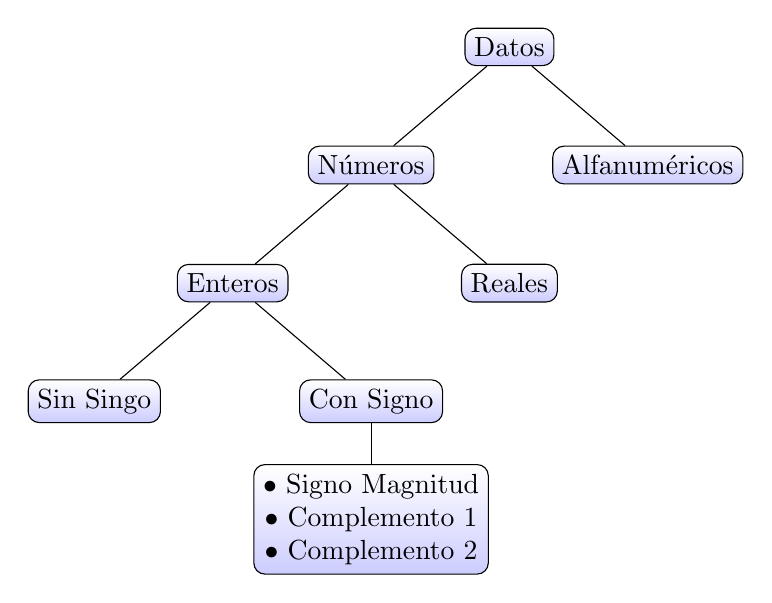
\begin{tikzpicture}[sibling distance=10em,
  every node/.style = {shape=rectangle, rounded corners,
    draw, align=center,
    top color=white, bottom color=blue!20}]]
  \node {Datos}
    child { node {Números} 
  	  child { node {Enteros}
  	  	child { node {Sin Singo}}
  	  	child { node {Con Signo}
			child { node {
			$\bullet$ Signo Magnitud\\
			$\bullet$ Complemento 1\\
			$\bullet$ Complemento 2
			}}  	  	
  	  	}
  	  }
        child { node {Reales}}  	  
  	  }
    child { node {Alfanuméricos}};
\end{tikzpicture}
\caption{Datos en un Computador}
\end{figure}
\section{Introducción al Lenguaje de Programación Ensamblador}
\section*{Miscelaneo}
\begin{center}
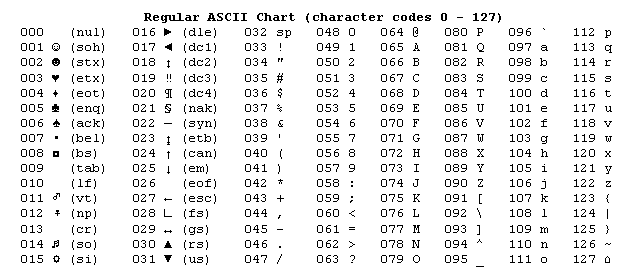
\includegraphics[scale=0.75]{ASCII}
\end{center}